\documentclass[12pt,a4paper]{article}
\usepackage[lmargin=3cm, tmargin=3cm, rmargin=2cm, bmargin=2cm]{geometry}
\usepackage{sbc-template}
\usepackage{graphicx,url}
\usepackage[utf8]{inputenc}  
\usepackage{ragged2e}
\usepackage{setspace}
\onehalfspacing
\setlength{\parindent}{1.25cm}
\usepackage{indentfirst}
\usepackage{graphicx}
\usepackage{float}
\usepackage{url}
\usepackage[brazil]{babel}
\usepackage{hyperref}
\sloppy

\title{Proposta inicial: CTP Acolhe}

\author{Isabela C. Silva, Jéssica S. Silva, Kaio Victtor Galvão, Maria Eduarda Lúcio,\\ Matheus S. Portes, Nickolas T. Silva, Werônica A. Melo }

\address{Instituto Federal de Educação, Ciência e Tecnologia de São Paulo (IFSP)\\
 São Paulo -- SP -- Brasil \\\
  Curso Técnico em Informática Integrado ao Ensino Médio
\nextinstitute
  PDS - Prática para Desenvolvimento de Sistemas\\\\
}

\begin{document} 

\maketitle

\begin{abstract}
  "CTP Acolhe" aims to improve the contact of students with the CTP, which is a department of the IFSP that offers educational and psychological help to students. Therefore, the project focuses on making it possible for anyone to get the help they need in a simpler and more direct way, through a web system that will be responsible for managing the appointments with the psychologists and study organization.

\end{abstract}
     
\begin{resumo} 
  O "CTP Acolhe" visa melhorar o contato dos alunos com a CTP, que é um departamento do IFSP que oferece ajuda pedagógica e psicológica aos estudantes. Portanto, o projeto tem como objetivo possibilitar para qualquer pessoa a ajuda que precisa de uma maneira mais simples e direta, através de um sistema web que será responsável por gerenciar os atendimentos com os psicólogos e organização de estudos.
\end{resumo}
\newpage


\listoffigures

\newpage
\begin{description}
        \item \textbf{Lista de siglas e abreviaturas}\\
        \item PDS Prática para Desenvolvimento de Sistemas
        \item IFSP Instituto Federal de Educação, Ciência e Tecnologia de São Paulo
        \item CTP Cordenadoria Técnico-Pedagógica
        \item DSP Diretoria adjunta Sociopedagógica
        \item Nasa National Aeronautics and Space Administration
        \item HTML HyperText Markup Language
        \item CSS Cascading Style Sheets
        \item SVN SubVersion
\end{description}

\newpage

\tableofcontents


\newpage

\section{Introdução}
\pagestyle{plain}
\pagenumbering{arabic}

Este documento expõe a proposta inicial do projeto de planejamento e execução de um sistema Web que será desenvolvido por meio da disciplina de \textit{PDS (Prática para Desenvolvimento de Sistemas)}, e através dos conhecimentos adquiridos ao longo dos anos de curso Técnico em Informática integrado ao Ensino Médio no IFSP. Também se trata de um projeto de conclusão de curso.
\indent

A equipe Lotus passou por um processo de levantamento de ideias, buscando projetos que fossem viáveis, se encaixassem nas exigências da disciplina de PDS, além de contribuírem para solucionar problemas encontrados no dia a dia. Pensando nisso, chegamos aos problemas presentes no IFSP.
\indent

Diversas são as adversidades que os estudantes do Instituto Federal do Câmpus São Paulo encontram diariamente, e entre elas, está o processo de contato com a \textit{CTP (Coordenadoria Técnico-Pedagógica)}. Ela atua acolhendo dúvidas e solicitações da comunidade escolar, disponibilizando orientações técnicas ao corpo discente, além de oferecer atendimentos individuais e/ou em grupos, com orientação e acompanhamento pedagógico e psicológico (no âmbito da Psicologia Escolar). 
\indent

O contato com a CTP, costuma ser realizado apenas presencialmente ou através de e-mail, não sendo um meio de comunicação tão prático. Além disso, muito alunos da Instituição não conhecem a CTP, nem os serviços e suporte que ela oferece, o que impossibilita que o estudante receba ajuda diante de suas dificuldades com a rotina escolar. 

\indent
Assim, o CTP Acolhe, busca tornar a comunicação e o conhecimento da Coordenadoria Técnico-Pedagógica mais acessível aos alunos do Instituto Federal do Câmpus São Paulo. Além de ajudar nos processos internos da CTP, possibilitando mais qualidade e conforto para os estudantes e funcionários.  

\subsection{Justificativa}

Durante o período de divulgação da pesquisa que deu iniciativa ao projeto obtivemos um total de 26 respostas, das quais, efetuadas por somente alunos matriculados no Instituto Federal de São Paulo, atenderam um total de 8 perguntas principais. Por intermédio desta, é perceptível e afirmável que 80,8\% dos entrevistados já sentiram dificuldades no que diz respeito a organização de seus estudos (Figura~\ref{fig01}).

\begin{figure}[H]
    \centering
    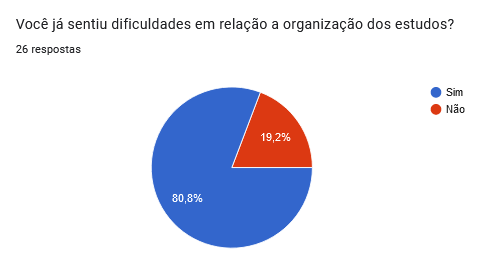
\includegraphics[width=14cm]{img1.png}
    \caption{Discentes que já sentiram dificuldades em relação a organização de seus estudos}
    \label{fig01}
\end{figure}

Ao ser questionado, pudemos concluir que mais discentes entrevistados estiveram predispostos do que não
tendentes a precisar de suporte psicológico para lidar com a situação de pressão estudantil no Campus São
Paulo durante algum período da sua extensão acadêmica (Figura~\ref{fig02}). 

\begin{figure}[H]
    \centering
    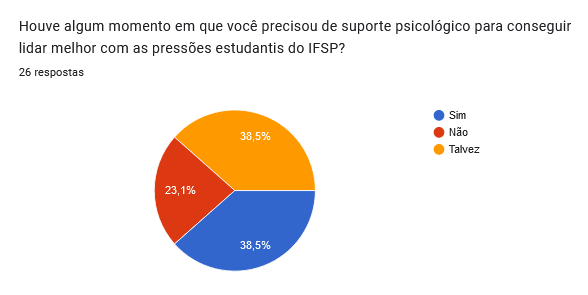
\includegraphics[width=15cm]{img2.png}
    \caption{Necessidade de suporte psicológico para lidar com as pressões estudantis no IFSP}
    \label{fig02}
\end{figure}

Apesar da maior parte dos estudantes demonstrarem indiretamente carência de engenhos proporcionados por serviços assegurados pela Coordenadoria Técnico-Pedagógica (CTP); A grande maioria, isto é, 76,9\% dos discentes, nunca tentaram entrar em contato com a CTP (Figura~\ref{fig03}).

\begin{figure}[H]
    \centering
    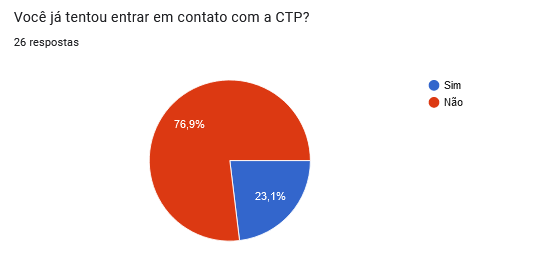
\includegraphics[width=14cm]{img3.png}
    \caption{Entrevistados que tentaram entrar em contato com a CTP}
    \label{fig03}
\end{figure}

O baixo índice de diligência no sentido de estabelecer contato com a \textit{Coordenadoria Técnico-Pedagógica (CTP)}. pode ser explicado pela falta de divulgação da atuação do setor Sociopedagógico do Câmpus e pela dificuldade encontrada por parte dos alunos na busca pelo serviço disponibilizado pela CTP.

Após indagar aos estudantes o que eles estimavam de uma plataforma que tivesse intuito de facilitar o contato entre o aluno e a \textit{Coordenadoria Técnico-Pedagógica (CTP)}, obtivemos que 88,5\% das respostas julgaram como uma plataforma necessária. Enquanto nenhuma afirmou não gostar da ideia (Figura~\ref{fig04}).

\begin{figure}[H]
    \centering
     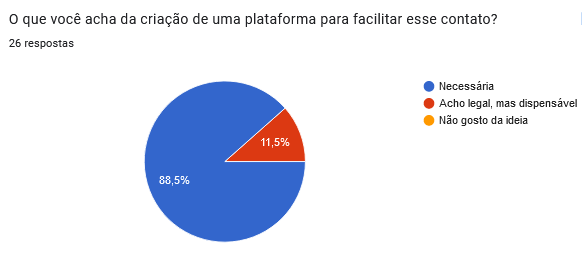
\includegraphics[width=15cm]{img4.png}
    \caption{Entrevistados que consideram como necessária a criação da plataforma}
    \label{fig04}
\end{figure}

Possuindo esses dados em mente, se faz importante a criação de um sistema (aplicação web) que facilite a comunicação entre o estudante do IFSP e a \textit{Coordenadoria Técnico-Pedagógica (CTP)}; para qual ajude os alunos que apresentam essa necessidade e sentem dificuldade de estabelecer contato ou entender o funcionamento do setor; além de organizar a demanda que chega para a CTP em função dos processos e incidentes.

Além disso, em ciência após diálogo com a \textit{Coordenadoria Técnico-Pedagógica (CTP)}, atualmente não chegam somente inquisições acerca de acompanhamentos psicológicos, mas também de dúvidas mais gerais que geralmente são tratadas por outro setor e de uma outra forma, uma vez que a CTP integra também a \textit{Diretoria adjunta Sociopedagógica (DSP)}. 

Assim também o faz necessário, pois é capaz de organizar os processos que chegam para a \textit{Coordenadoria Técnico-Pedagógica (CTP)}, minando qualquer tipo de atraso ou confusão no momento de atender as exigências e estabelecer ordem de importância para tais.


\subsection{Objetivo}

O projeto CTP Acolhe tem como objetivo facilitar a comunicação direta entre os alunos e a \textit{CTP (Coordenadoria Técnico-Pedagógica)}, centralizando esses incidentes, ao mesmo tempo que divulga o seu apoio pedagógico e psicológico aos estudantes.

Além disso, por meio de perguntas e respostas, colheremos informações iniciais importantes para caracterizar cada incidente, com o intuito de melhorar a organização desses incidentes por prioridades, de acordo com requisitos que ainda serão discutidos com a CTP durante o desenvolvimento do projeto.

No entanto, ainda sim, buscamos passar confiança e segurança aos alunos que buscarem ajuda através do CTP Acolhe, pois, ainda que seja normal precisar de ajuda, muitos alunos podem sentir medo de serem expostos ou se sentirem vulneráveis ao entrar em contato com psicólogos do IFSP.

\section{Proposta}

CTP Acolhe, tem como proposta inicial a criação de um website que aproximará os estudantes do IFSP à Coordenadoria Técnico-Pedagógica através de incidentes. Tendo algumas funcionalidades principais como:

\textbf{Chatbot:} O Chatbot será primordial na criação do incidente do aluno,  sendo dividido em casos  referentes a ajuda psicológica ou ajuda organizacional. Nele o aluno entrará em uma conversa com um bot que mostrará opções durante a conversa e, dependendo das suas repostas, criará um evento para os psicólogos. Caso a resposta que o aluno registrou dê indícios de um caso que necessita de mais atenção, esse incidente ficará marcado como prioritário para os psicólogos.

\textbf{Questionário:} Quando o estudante entra na plataforma, é exibido na tela um questionário perguntando como ele está naquele dia –“carinha sorridente, carrinha feliz, carinha normal, carinha triste”. A resposta que o estudante por nesse questionário será exibida para os psicólogos e, caso ponha uma resposta de “carinha triste” criará um alerta para esse aluno. O aluno poderá responder esse questionário apenas uma vez no dia, porém, todos os dias ele aparecerá para ser respondido. Essa atribuição ajudará os psicólogos no acompanhamento periódico dos estudantes.

\textbf{Lista de casos organizados por prioridade:} Os incidentes que a CTP acompanhará ficarão organizados em listas, sendo divididos em prioridades de casos. O que irá definir a ordem de atendimento do psicólogo é a gravidade do incidente, o horário em que ele é criado e os registros do questionário.

Com o incidente criado, o psicólogo agendará um atendimento ao aluno à fim de entender suas necessidades e dores.

\section{Tecnologias e ferramentas}

Uma das etapas mais importantes no processo de desenvolvimento de um sistema é a escolha das tecnologias que vão ser utilizadas. Numa era com mudanças tão rápidas, principalmente no setor informático e tecnológico, é preciso que as escolhas sejam feitas com uma visão de longo prazo, na tentativa de acompanhar as tendências do mercado para que o produto não se torne ultrapassado em questão de poucos anos. Além do dilema da durabilidade das tecnologias escolhidas, estas também devem atender às necessidades do projeto, de forma que tudo o que se te pretende fazer possa ser desenvolvido sem maiores dificuldades. Portanto, é essencial que uma análise o mais completa possível seja feita em relação ao mercado e às necessidades do projeto. Assim, estas foram as tecnologias escolhidas para o desenvolvimento deste projeto:

\begin{enumerate}
    \item Banco de dados
\begin{description}
    \item a) MySql: A princípio, a utilização do MySQL era destinada a projetos de pequeno e médio porte, mas atualmente ele consegue suportar muito mais registros e processamentos. É um sistema de fácil emprego, com constantes atualizações, além de ser usado por empresas de renome que possuem um volume de dados gigante, tais como Bradesco, Sony e a própria NASA. Por ser desenvolvido em C e C++, é compatível com diversos sistemas operacionais, a citar os mais importantes do mercado atualmente: Windows, Linux e Mac OS X Server. Ele também possui interface para várias linguagens, incluindo as que serão utilizadas neste projeto; além de alta velocidade, uma já citada grande capacidade de execução e armazenamento, e utilização de SQL, que é a linguagem mais utilizada quando se fala em banco de dados.   Ademais, ele é o segundo Sistema de Gerenciamento de Banco de Dados (SGBD)\cite{artigo2} mais popular do mundo segundo o DB-Engines , principal ranking do assunto; e o primeiro segundo a pesquisa “Tecnologias mais populares de 2022”\cite{artigo4}, realizada pelo StackOverflow\cite{artigo3} . Outrossim, é uma ferramenta com a qual já se tem muita familiaridade.\\\\
\end{description}

    \item Back-End
\begin{description}
    \item a) Java: Criada pela  \textit{Sun Microsystems} e posteriormente adquirida pela Oracle, o Java tornou-se um gigante no desenvolvimento de aplicações. É uma linguagem orientada a objetos e tem como foco alta performance, portabilidade — pode ser o código pode ser escrito uma só vez e rodado em diversos dispositivos —, e segurança\cite{artigo}.  Além disso, o Spring, framework mais popular quando se fala de Java, também será utilizado, visto que poupa tempo quando se fala de configuração e padronização, dando mais foco ao desenvolvedor para o desenvolvimento em si do que para a infraestrutura do projeto. Analisando o mercado, o Java está entre as dez linguagens de programação, scripting e marcação mais populares segundo a pesquisa “Tecnologias mais populares de 2022”, já citada; e o Spring está entre os cinco frameworks mais populares. O Java e seu framework, Spring, já foram utilizados em projetos anteriores.\\
\end{description}

  \item Front-End
\begin{description}
   \item a) HTML: O \textit{HyperText Markup Language (HTML)} é uma linguagem de marcação vastamente utilizada no desenvolvimento web, tornando-se indispensável para qualquer projeto que siga este objetivo. É um dos pilares para a estruturação da interface do sistema, além de muito conhecida no mercado e por nós.\\

    \item b) CSS: O \textit{Cascading Style Sheets (CSS)} é uma linguagem de estilização, responsável pela personalização dos elementos marcados pelo HTML: cores, fontes, tamanhos etc. são todos definidos por esta linguagem. Ademais, ela já está muito consolidada no mercado, tem uma facílima integração com as outras linguagens escolhidas e compõe a nossa experiência.\\

    \item c) JavaScript: Ao lado do HTML e do CSS, o JavaScript lidera o ranking de linguagens de programação, scripting e marcação da pesquisa já citada do StackOverflow, formando o trio de linguagens mais populares no desenvolvimento web atualmente. É uma linguagem de programação de alto nível intensamente utilizada para fornecer dinamicidade e interação de elementos dentro de uma página. Por fim, também já foi utilizada por nós.\\

    \item d) React.js: O React é uma biblioteca JavaScript que possibilita que certos elementos de uma página possam ser separados em componentes reutilizáveis. Assim sendo, um botão pode ser desenvolvido uma única vez para ser utilizado em inúmeras páginas do mesmo projeto. Além disso, ele fornece mais dinamicidade ainda à interface, graças à sua administração de estado, que permite que algumas informações sejam passadas entre diversos componentes para suas respectivas atualizações apenas se for necessário, não havendo necessidade de atualizar a página inteira. Criada em 2011 pelo Facebook, o React hoje, segundo o StackOverflow, está entre as principais tecnologias web, perdendo apenas para o Node.js. Alguns de nós já utilizaram esta tecnologia e conhecem seu funcionamento.\\
\end{description}

    \item Versionamento
    \begin{description}
        \item a) SubVersion: O \textit{SubVersion  (SVN)} é um controlador de versão que gerencia arquivos e diretórios, tornando possível visualizar o histórico de alterações, os autores dessas alterações e sua recuperação. É muito proveitoso para trabalhar em grupo, visto que muitos usuários podem fazer suas modificações sempre que necessário. Esta ferramenta foi escolhida porque é uma obrigatoriedade da matéria de PDS.\\
    \end{description}

    \item Documentação
    \begin{description}
        \item a) \LaTeX: O \LaTeX  é um sistema de composição que permite que documentos sejam criados num formato predeterminado sem que haja grandes dificuldades de configuração. Para tanto, utilizaremos o Overleaf, que permite a criação de documentos, relatórios, projetos etc. a partir do emprego do \LaTeX. Esta ferramenta também foi escolhida por ser uma obrigatoriedade da matéria de PDS, além de permitir que todos os integrantes tenham acesso à edição do mesmo documento.
    \end{description}
\end{enumerate}

\section{Equipe}
A equipe Lotus é composta por sete integrantes, cada um deles possuindo habilidades que foram adquiridas ao longo do curso de Informática, skills estas que serão utilizadas para realizar o projeto CTP Acolhe. Pela grande gama de conhecimentos diferentes, há uma distribuição de tarefas com intuito de aproveitar melhor cada aptidão e disponibilidade dos integrantes, se adequando ás necessidades do projeto.

\subsection{Divisão dos membros}
Isabela Cruz: A integrante Isabela atuará como gerente de mídias do CTP Acolhe, coordenando os Posts do Blog e das demais redes sociais da Lotus. Além disso, também estará participando da elaboração do Documento do projeto.

Jéssica Sobral: A Jéssica atuará como uma full-stack no projeto, dando suporte no desenvolvimento do Front e Back-end da aplicação. Ademais, será Coordenadora do desenvolvimento do Banco de Dados, juntamente do Matheus Portes, além de contribuir com a documentação.

Kaio Victtor: O membro Kaio Victtor será coordenador do desenvolvimento Front-end do CTP Acolhe, atuando na produção da interface do sistema. Bem como auxiliará nas mídias, gerencia do projeto e documentação.

Maria Lucio: A Maria lúcio será a Coordenadora geral do projeto, ela ficará à cargo de realizar as pesquisas de campo bem como gerir o desenvolvimento como todo. Somando ainda à sua participação da elaboração do Documento.

Matheus Portes: O Matheus Portes atuará juntamente com a Jessíca Sobral na coordenação do banco de dados, além de auxiliar o desenvolvimento front e back-end do CTP Acolhe, bem como sua participação na elaboração do documento. 

Nickolas Tavares: O integrante Nickolas Tavares será o coordenador  back-end da aplicação, bem como atuará também na manutenção do banco de dados. Fora isto, também participará da escrita da documentação.

Werônica Melo: A Weronica Melo será a coordenadora da Documentação do projeto, ela quem ira gerir e fazer a verificação da escrita do documento. Para mais, também atuará como suporte de mídias da Lotus.

\subsection{Divisão de tarefas}
As tarefas foram divididas de acordo com a área de interesse e competência de cada componente da Lotus. Sendo assim, há uma grande distribuição de atividades visando melhorar o fluxo do desenvolvimento. Ademais  documentação fica a cargo de todos os elementos da equipe, por conta da interdisciplinaridade de cada ofício.

 O quadro da distribuição foi feito da seguinte forma (Figura~\ref{fig05}):
\begin{figure}[H]
    \centering
     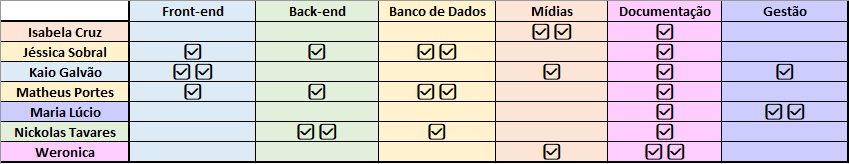
\includegraphics[width=15cm]{img5.png}
    \caption{Cada área há um gerente ou mais para se responsabilizar quanto ao desenvolvimento de cada parte do projeto.}
    \label{fig05}
\end{figure}

\newpage

\bibliographystyle{plain}
%\bibliographystyle{abntex2-alf}
\bibliography{sbc-template}

\newpage
\section{Glossário}
\indent
        Sistema Web 
        Um tipo de site dinâmico hospedo na internet, possibilitando o acesso em qualquer lugar através de dispositovos que tenham um nagevador e internet.
    
         StackOverflow 
        Uma comunidade que ajuda a auxiliar desenvolvedores, através de dúvidas sobre os processos de desenvolvimento.
        
        Overleaf
        Uma plataforma para edição de texto Latex, que facilita o processo de realização de documentos acadêmicos.
        
         Skills 
        Conjunto de habilidades e capacidades que são adquiridas ao longo dos anos, ou por um período de tempo.
        
        Framework 
        Uma abstração que une códigos comuns entre outros projetos de software provendo uma funcionalidade genérica.
        
\newpage

\section{Apêndices}
\subsection{Apêndice A - Pesquisa de campo}

\begin{figure}[H]
    \centering
     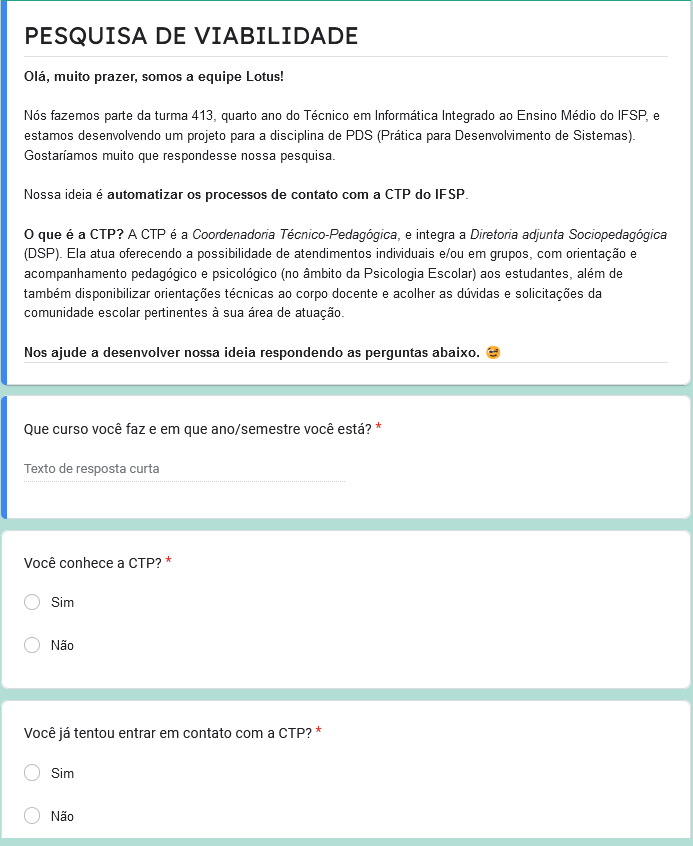
\includegraphics[width=15cm]{foto1.png}
\end{figure}

\begin{figure}[H]
    \centering
     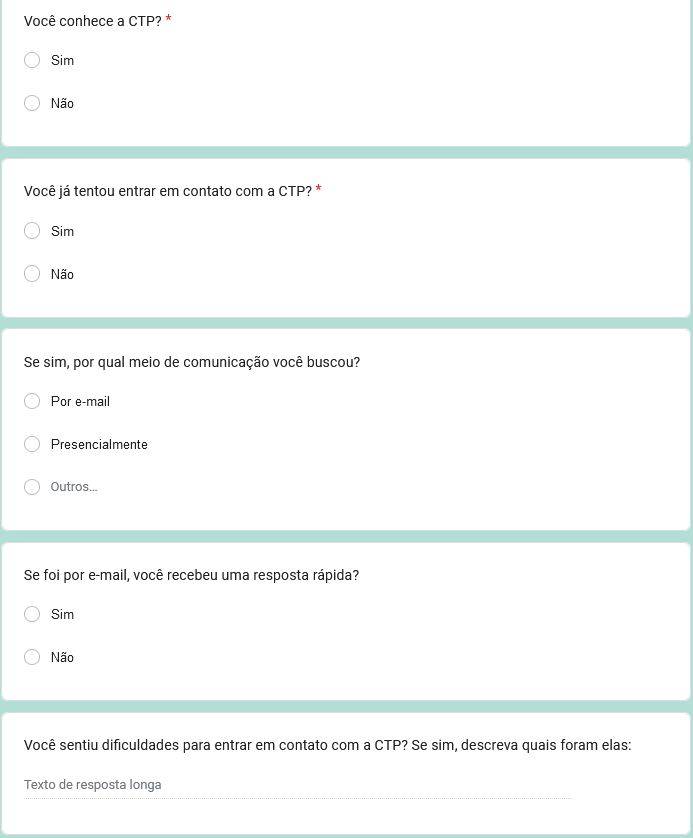
\includegraphics[width=15cm]{foto2.png}
\end{figure}

\begin{figure}[H]
    \centering
     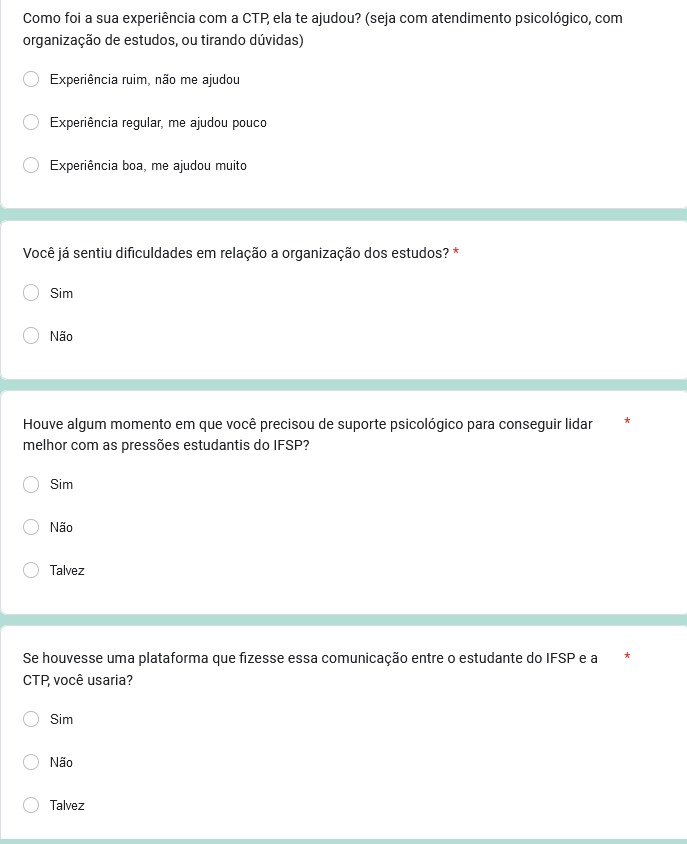
\includegraphics[width=15cm]{foto3.png}
\end{figure}

\begin{figure}[H]
    \centering
     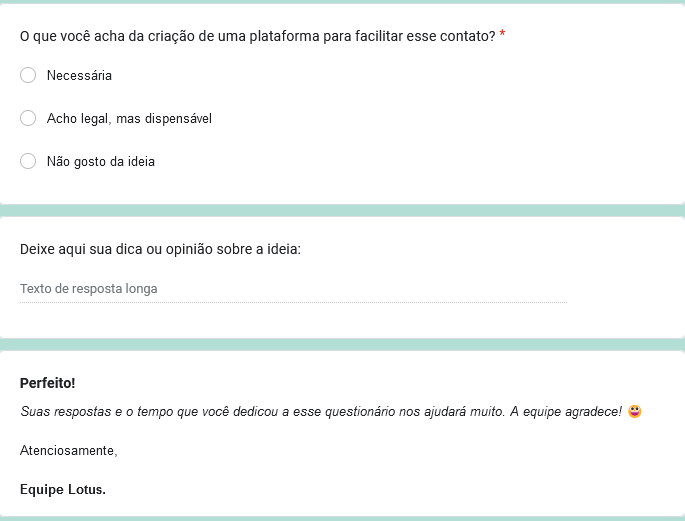
\includegraphics[width=15cm]{foto4.png}
     \caption{Pesquisa de campo}
     \label{fig06}
\end{figure}

\subsection{Apêndice B  - Atas de reuniões}
\begin{figure}[H]
    \centering
     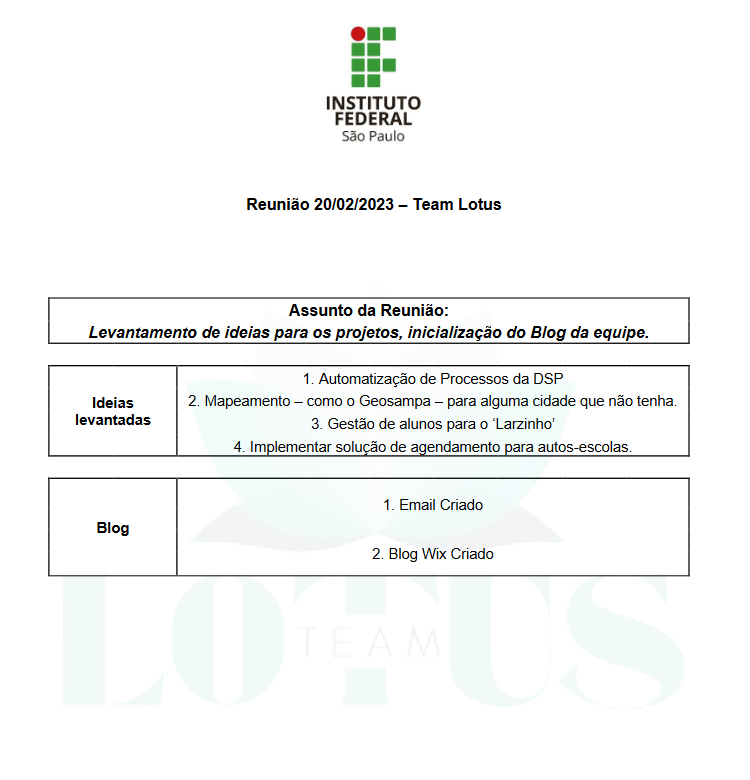
\includegraphics[width=15cm]{ilus1.png}
     \caption{Primeira reunião}
     \label{fig07}
\end{figure}

\begin{figure}[H]
    \centering
     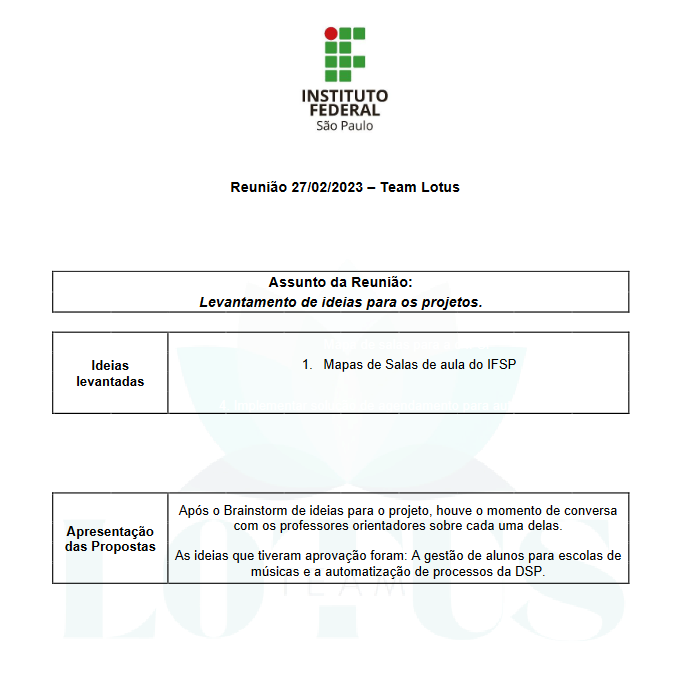
\includegraphics[width=15cm]{ilus2.png}
     \caption{Segunda reunião}
     \label{fig08}
\end{figure}

\begin{figure}[H]
    \centering
     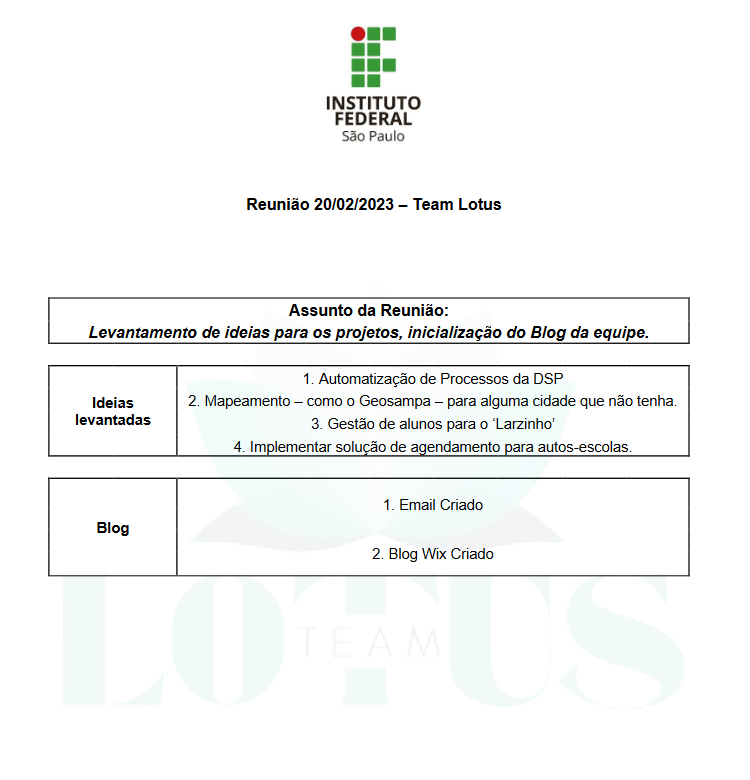
\includegraphics[width=15cm]{ilus1.png}
     \caption{Terceira reunião}
     \label{fig09}
\end{figure}


\end{document}

